\documentclass{article}

\usepackage[utf8]{inputenc}
\usepackage{enumitem}
\usepackage{float}
\usepackage{circuitikz}
\usepackage{todonotes}
\usepackage{amsmath}
\usepackage{tikz}
\usetikzlibrary{shapes, calc, shapes, arrows}
\usepackage{svg}


\title{Blatt 3}
\author{Luca Krüger, Jonas Otto, Jonas Merkle (Gruppe R)}
\date{\today}

\begin{document}
\maketitle

\section{Lernregeln}
$$E(w,b)=\frac{1}{2}\sum_{\mu=1}^{M}(T_{\mu}-f(wx_{\mu}+b))^2$$
\begin{enumerate}
  \item
        \begin{align*}
          \nabla E(w,b)=\begin{pmatrix} \dfrac{\strut \partial E}{\strut \partial w} \\ \dfrac{\strut \partial E}{\strut \partial b}\end{pmatrix} = \begin{pmatrix}
            - \sum_{\mu=1}^{M}(T_{\mu}-f(wx_{\mu}+b)) \cdot f'(wx_{\mu}+b)\cdot x_{\mu} \\
            - \sum_{\mu=1}^{M}(T_{\mu}-f(wx_{\mu}+b)) \cdot f'(wx_{\mu}+b)
          \end{pmatrix} \\
        \end{align*}
  \item
        \begin{enumerate}[label=\alph*)]
          \item inkrementelle Version:
                \begin{align*}
                  w(t+1) & =w(t)-\eta(T_{t}-f(wx_{t}+b)) \cdot f'(wx_{t}+b)\cdot x_t \\
                  b(t+1) & =b(t)-\eta(T_{t}-f(wx_{t}+b)) \cdot f'(wx_{t}+b)
                \end{align*}
          \item Batch Version:
                \begin{align*}
                  w(t+1) & =w(t)+\eta\sum_{\mu=1}^{M}(T_{\mu}-f(wx_{\mu}+b)) \cdot f'(wx_{\mu}+b)\cdot x_{\mu} \\
                  b(t+1) & =b(t)+\eta\sum_{\mu=1}^{M}(T_{\mu}-f(wx_{\mu}+b)) \cdot f'(wx_{\mu}+b)
                \end{align*}
        \end{enumerate}
  \item
        \begin{enumerate}[label=\alph*)]
          \item (Siehe Jupyter Notebook)
          \item Negativer Gradient (\textit{blau}) im initialen Punkt $\begin{pmatrix}w(0) \\ b(0)\end{pmatrix} = \begin{pmatrix} -1 \\ 3 \end{pmatrix}$ :
                \begin{figure}[H]
                  % body of the figure
                  \centering
                  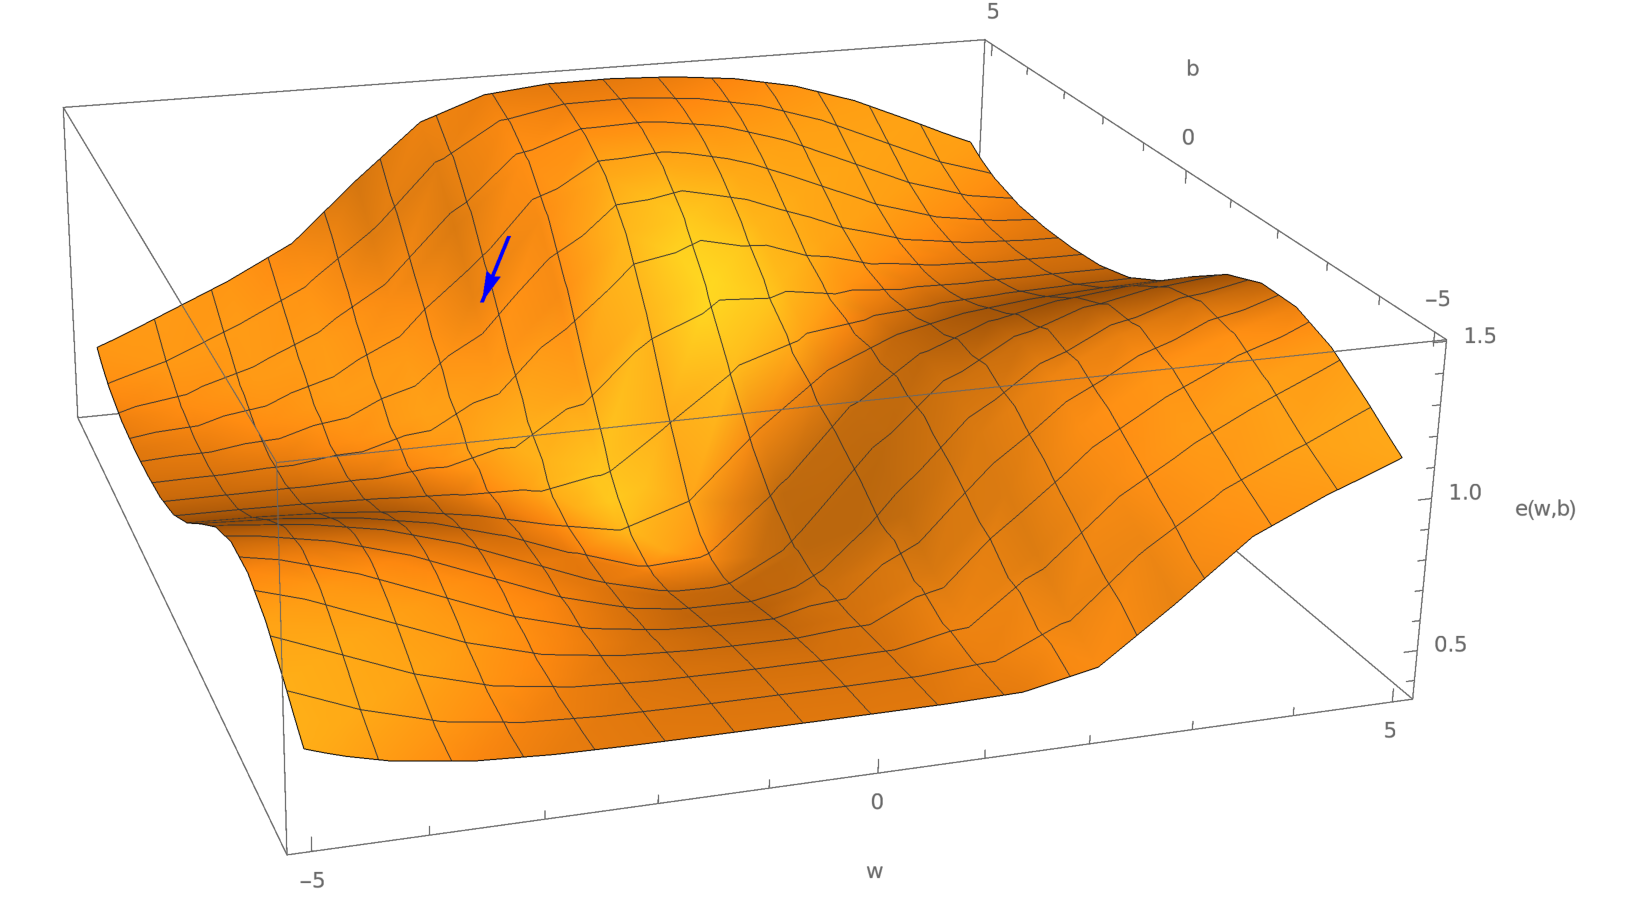
\includegraphics[width=\textwidth]{initial-error-gradient.pdf}
                  \caption{Gradient bei $t=0$}
                \end{figure}

          \item (Siehe Jupyter Notebook)
          \item Der Pfad in Abbildung 3 auf dem Übungsblatt verläuft vom Startpunkt in ein lokales Minimum der Errorfunktion mit hohen Werten für $w$ und $b$.  Problematisch an der Gradienten-Lernregel $E(t)$ ist, dass im Allgemeinen gilt $E(t_1)>E(t_2)$ für zwei aufeinanderfolgende Lernschritte $t_1, t_2$ und somit ein Minimum nur in einer lokal monoton fallenden Umgebung des Startpunktes gefunden werden kann. D.h., der Endpunkt des Pfades hängt bei der Lernregel stark von den Anfangswerten ab und ein gefundendes Minimum ist nicht zwangsweise ein globales Minimum der Errorfunktion.
        \end{enumerate}
  \item
        \begin{enumerate}[label=\alph*)]
          \item \textit{Pfad} 1 wurde mit der Batch-Lernregel und \textit{Pfad 2} mit der inkrementellen Lernregel erzeugt. Der Gradient von \textit{Pfad 1} ist im Gegensatz zu \textit{Pfad 2} eine stetige Funktion, da in jedem Lernschritt die Errorfunktion über den gesamten Trainingsdatensatz berechnet wurde. Für die inkrementelle Lernregel, wird in jedem Lernschritt die Errorfunktion nur über ein Element aus dem Trainingtsdatensatz berechnet.
          \item Die Lernregel über alle Datenpunkte ist insbesondere bei größeren Datensätzen sehr zeitintensiv. Die inkrementelle Lernregel gewichtet einzelne Extremwerte im Datensatz möglicherweise zu stark.
        \end{enumerate}
  \item Wenn die Lernrate sehr groß gewählt wird, erreicht der Fehler zwar schnell eine Umgebung des Minimums, springt dann aber über das Minimum und oszilliert um das Minimum herum oder divergiert sogar.
  \item Die Werte sind nicht linear separierbar, das Klassifizierungsproblem kann also von diesem Netz nicht gelöst werden.
\end{enumerate}



\end{document}
